\documentclass[]{article}
\usepackage{lmodern}
\usepackage[compact]{titlesec}
\usepackage{amssymb,amsmath}
\usepackage{ifxetex,ifluatex}
\usepackage{fixltx2e} % provides \textsubscript
\ifnum 0\ifxetex 1\fi\ifluatex 1\fi=0 % if pdftex
  \usepackage[T1]{fontenc}
  \usepackage[utf8]{inputenc}
\else % if luatex or xelatex
  \ifxetex
    \usepackage{mathspec}
  \else
    \usepackage{fontspec}
  \fi
  \defaultfontfeatures{Ligatures=TeX,Scale=MatchLowercase}
\fi
% use upquote if available, for straight quotes in verbatim environments
\IfFileExists{upquote.sty}{\usepackage{upquote}}{}
% use microtype if available
\IfFileExists{microtype.sty}{%
\usepackage{microtype}
\UseMicrotypeSet[protrusion]{basicmath} % disable protrusion for tt fonts
}{}
\usepackage[margin=1in]{geometry}
\usepackage{hyperref}
\hypersetup{unicode=true,
            pdftitle={Maps},
            pdfauthor={Darryl Buswell},
            pdfborder={0 0 0},
            breaklinks=true}
\urlstyle{same}  % don't use monospace font for urls
\usepackage{longtable,booktabs}
\usepackage{graphicx,grffile}
\makeatletter
\def\maxwidth{\ifdim\Gin@nat@width>\linewidth\linewidth\else\Gin@nat@width\fi}
\def\maxheight{\ifdim\Gin@nat@height>\textheight\textheight\else\Gin@nat@height\fi}
\makeatother
% Scale images if necessary, so that they will not overflow the page
% margins by default, and it is still possible to overwrite the defaults
% using explicit options in \includegraphics[width, height, ...]{}
\setkeys{Gin}{width=\maxwidth,height=\maxheight,keepaspectratio}
\IfFileExists{parskip.sty}{%
\usepackage{parskip}
}{% else
\setlength{\parindent}{0pt}
\setlength{\parskip}{6pt plus 2pt minus 1pt}
}
\setlength{\emergencystretch}{3em}  % prevent overfull lines
\providecommand{\tightlist}{%
  \setlength{\itemsep}{0pt}\setlength{\parskip}{0pt}}
\setcounter{secnumdepth}{0}
% Redefines (sub)paragraphs to behave more like sections
\ifx\paragraph\undefined\else
\let\oldparagraph\paragraph
\renewcommand{\paragraph}[1]{\oldparagraph{#1}\mbox{}}
\fi
\ifx\subparagraph\undefined\else
\let\oldsubparagraph\subparagraph
\renewcommand{\subparagraph}[1]{\oldsubparagraph{#1}\mbox{}}
\fi

%%% Use protect on footnotes to avoid problems with footnotes in titles
\let\rmarkdownfootnote\footnote%
\def\footnote{\protect\rmarkdownfootnote}

%%% Change title format to be more compact
\usepackage{titling}

% Create subtitle command for use in maketitle
\newcommand{\subtitle}[1]{
  \posttitle{
    \begin{center}\large#1\end{center}
    }
}

\setlength{\droptitle}{-2em}
  \title{Maps}
  \pretitle{\vspace{\droptitle}\centering\huge}
  \posttitle{\par}
\subtitle{MSPA PREDICT 455-DL-SEC55}
  \author{Darryl Buswell}
  \preauthor{\centering\large\emph}
  \postauthor{\par}
  \date{}
  \predate{}\postdate{}

\begin{document}
\maketitle

\newpage

\section{1 Introduction}\label{introduction}

This assignment explores Census data for United States, with the aim of
identifying trends or anomalies in the underlying data using both static
and animated choropleth maps.

\section{2 Data}\label{data}

Data for this assessment was obtained from the United States Census
Bureau (Commerce 2015). An API key was obtained and used in order to
pull relevant data from the the American Community Survey (ACS). This
data includes population, age and sex data for the United States from
2009. A list of tables queried as part of this assessment can be found
in Appendix A.

\section{3 Data Exploration}\label{data-exploration}

A choropleth maps provides a useful method for visualizing spatial data.
In R, perhaps the most simple method of generating a choropleth map is
to use the `choroplethr' package by Trulia (Innovation 2014). This
package is able to pass ACS data and build a relevant choropleth map in
a single R command.

We use the `state\_choropleth\_acs' command to generate a choropleth map
of the United States to show the population, median age and household
income for each state over the years 2009 to 2014. These figures are
shown in Appendix B. By default, `choroplethr' divides the lower 48
states into nine equally sized buckets and colors the buckets using a
sequential brewer scale. We see that states with the greatest population
over this period include California, Texas, Illinois, Ohio,
Pennsylvania, New York and Florida. Interestingly, these states also
have recorded the greatest household income over this period. In terms
of median age, Florida, West Virginia, Pennsylvania, Vermont and Maine
have a relatively greater median age than other states.

We can also look at the data at the county level by using the
`county\_choropleth\_acs' command. This gives us greater detail, however
there is a trade-off in terms of interpretability. That is, it can be
more difficult to attribute individual states as having a relatively
high or low characteristic, however we can see more broadly which
general areas have a relatively high or low characteristic. For example,
we generally see a greater population and higher level of income along
the east and west coast of the United States, while a lower population
and level of income within central United States.

The `choroplethr' package does provide some flexibility in terms of how
we categorize the data. We can for example, force the amount of data
buckets to two. This allows us to more easily recognize counties which
have a income level above or below a certain threshold. We can also zoom
on particular states. For example, we have generated a map which zooms
on states on the west coast of the United States (Washington, Oregon,
California, Idaho, Nevada, Utah and Arizon). Figures for these data
subsets are also shown in Appendix B.

Perhaps the most useful feature of the `choroplethr' package is its
ability to automatically generate an animated choropleth map. The
package does this by appending a number of maps to a list of
choropleth's, generating a choropleth map image for each, and
subsequently exporting these maps to a directory. The package will also
create a html file with a JavaScript based player that allows the viewer
to cycle through each choroplethr map. We have used this function to
generate a set of choropleth map's for population at the county level
within the United States, for five year periods ending 2009 through to
2014. The generated images and JavaScript player can be found within the
working directory of this markdown document.

\section{4 Conclusion}\label{conclusion}

We were able to leverage the `choroplethr' package in order to generate
a number of choropleth maps of ACS statistics for the United States.
This package allowed us to easily identify states which have a
relatively high or low population, median age and income. We were also
able to investigate some of the flexibility of this package by zooming
into particular states and creating an animated choropleth map of
population within the United States at a county level.

\newpage

\section{Appendix A Table Output}\label{appendix-a-table-output}

\subsubsection{Table A1 ACS Table Query}\label{table-a1-acs-table-query}

\begin{longtable}[]{@{}ll@{}}
\toprule
\begin{minipage}[b]{0.10\columnwidth}\raggedright\strut
Table
\strut\end{minipage} &
\begin{minipage}[b]{0.84\columnwidth}\raggedright\strut
Description
\strut\end{minipage}\tabularnewline
\midrule
\endhead
\begin{minipage}[t]{0.10\columnwidth}\raggedright\strut
B01002
\strut\end{minipage} &
\begin{minipage}[t]{0.84\columnwidth}\raggedright\strut
MEDIAN AGE BY SEX
\strut\end{minipage}\tabularnewline
\begin{minipage}[t]{0.10\columnwidth}\raggedright\strut
B01003
\strut\end{minipage} &
\begin{minipage}[t]{0.84\columnwidth}\raggedright\strut
TOTAL POPULATION
\strut\end{minipage}\tabularnewline
\begin{minipage}[t]{0.10\columnwidth}\raggedright\strut
B19001
\strut\end{minipage} &
\begin{minipage}[t]{0.84\columnwidth}\raggedright\strut
HOUSEHOLD INCOME IN THE PAST 12 MONTHS (IN 2012 INFLATION-ADJUSTED
DOLLARS)
\strut\end{minipage}\tabularnewline
\bottomrule
\end{longtable}

\newpage

\section{Appendix B Figure Output}\label{appendix-b-figure-output}

\subsubsection{Figure B1 United States Population by
State}\label{figure-b1-united-states-population-by-state}

\section{\texorpdfstring{\protect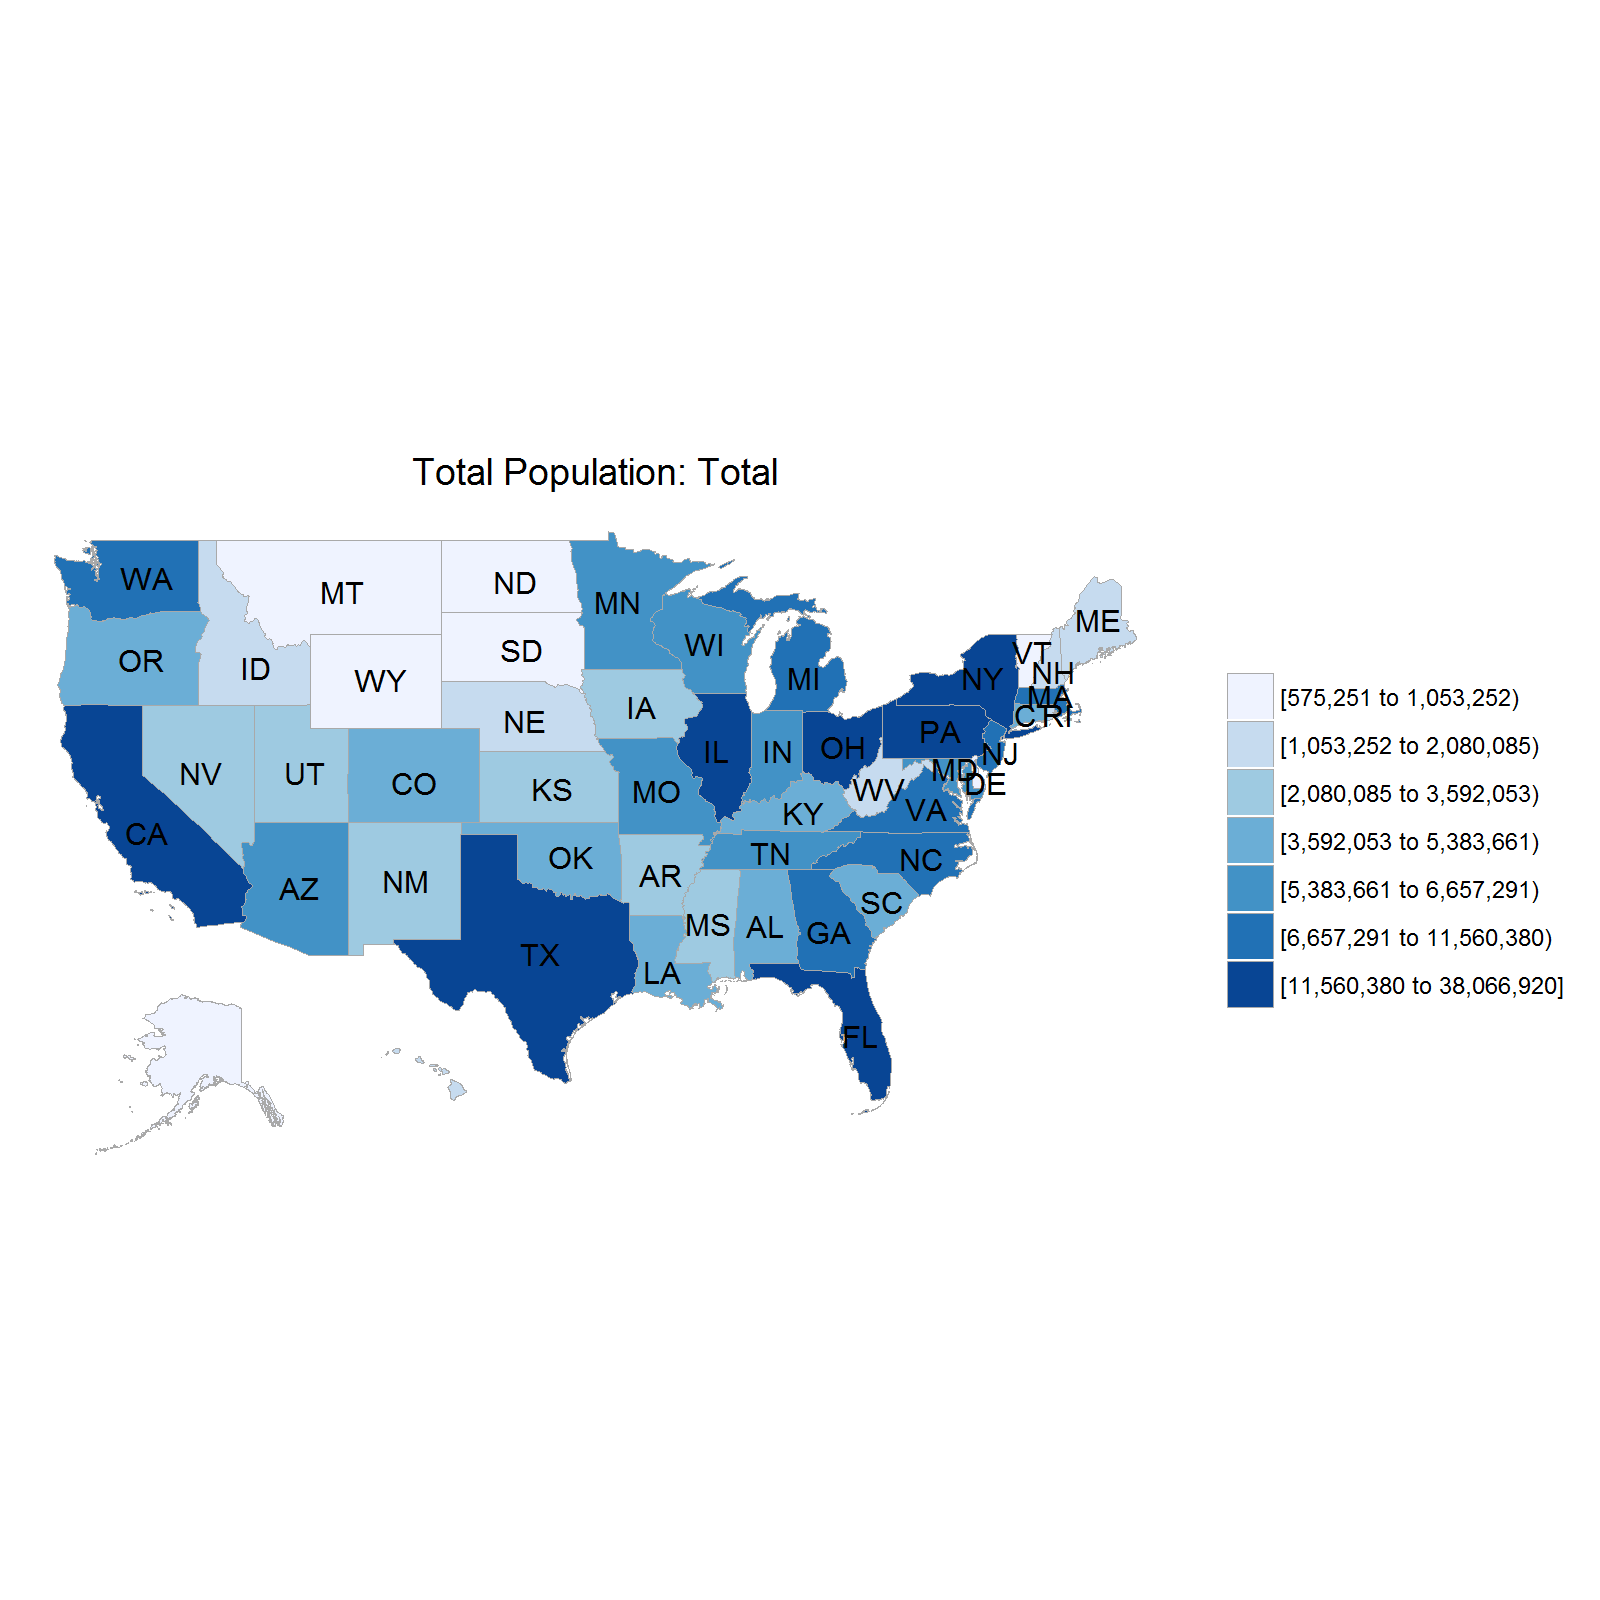
\includegraphics[height=12.50000in]{images/state_pop.png}}{US Population by State}}\label{us-population-by-state}

\newpage

\subsubsection{Figure B2 United States Median Age by
State}\label{figure-b2-united-states-median-age-by-state}

\section{\texorpdfstring{\protect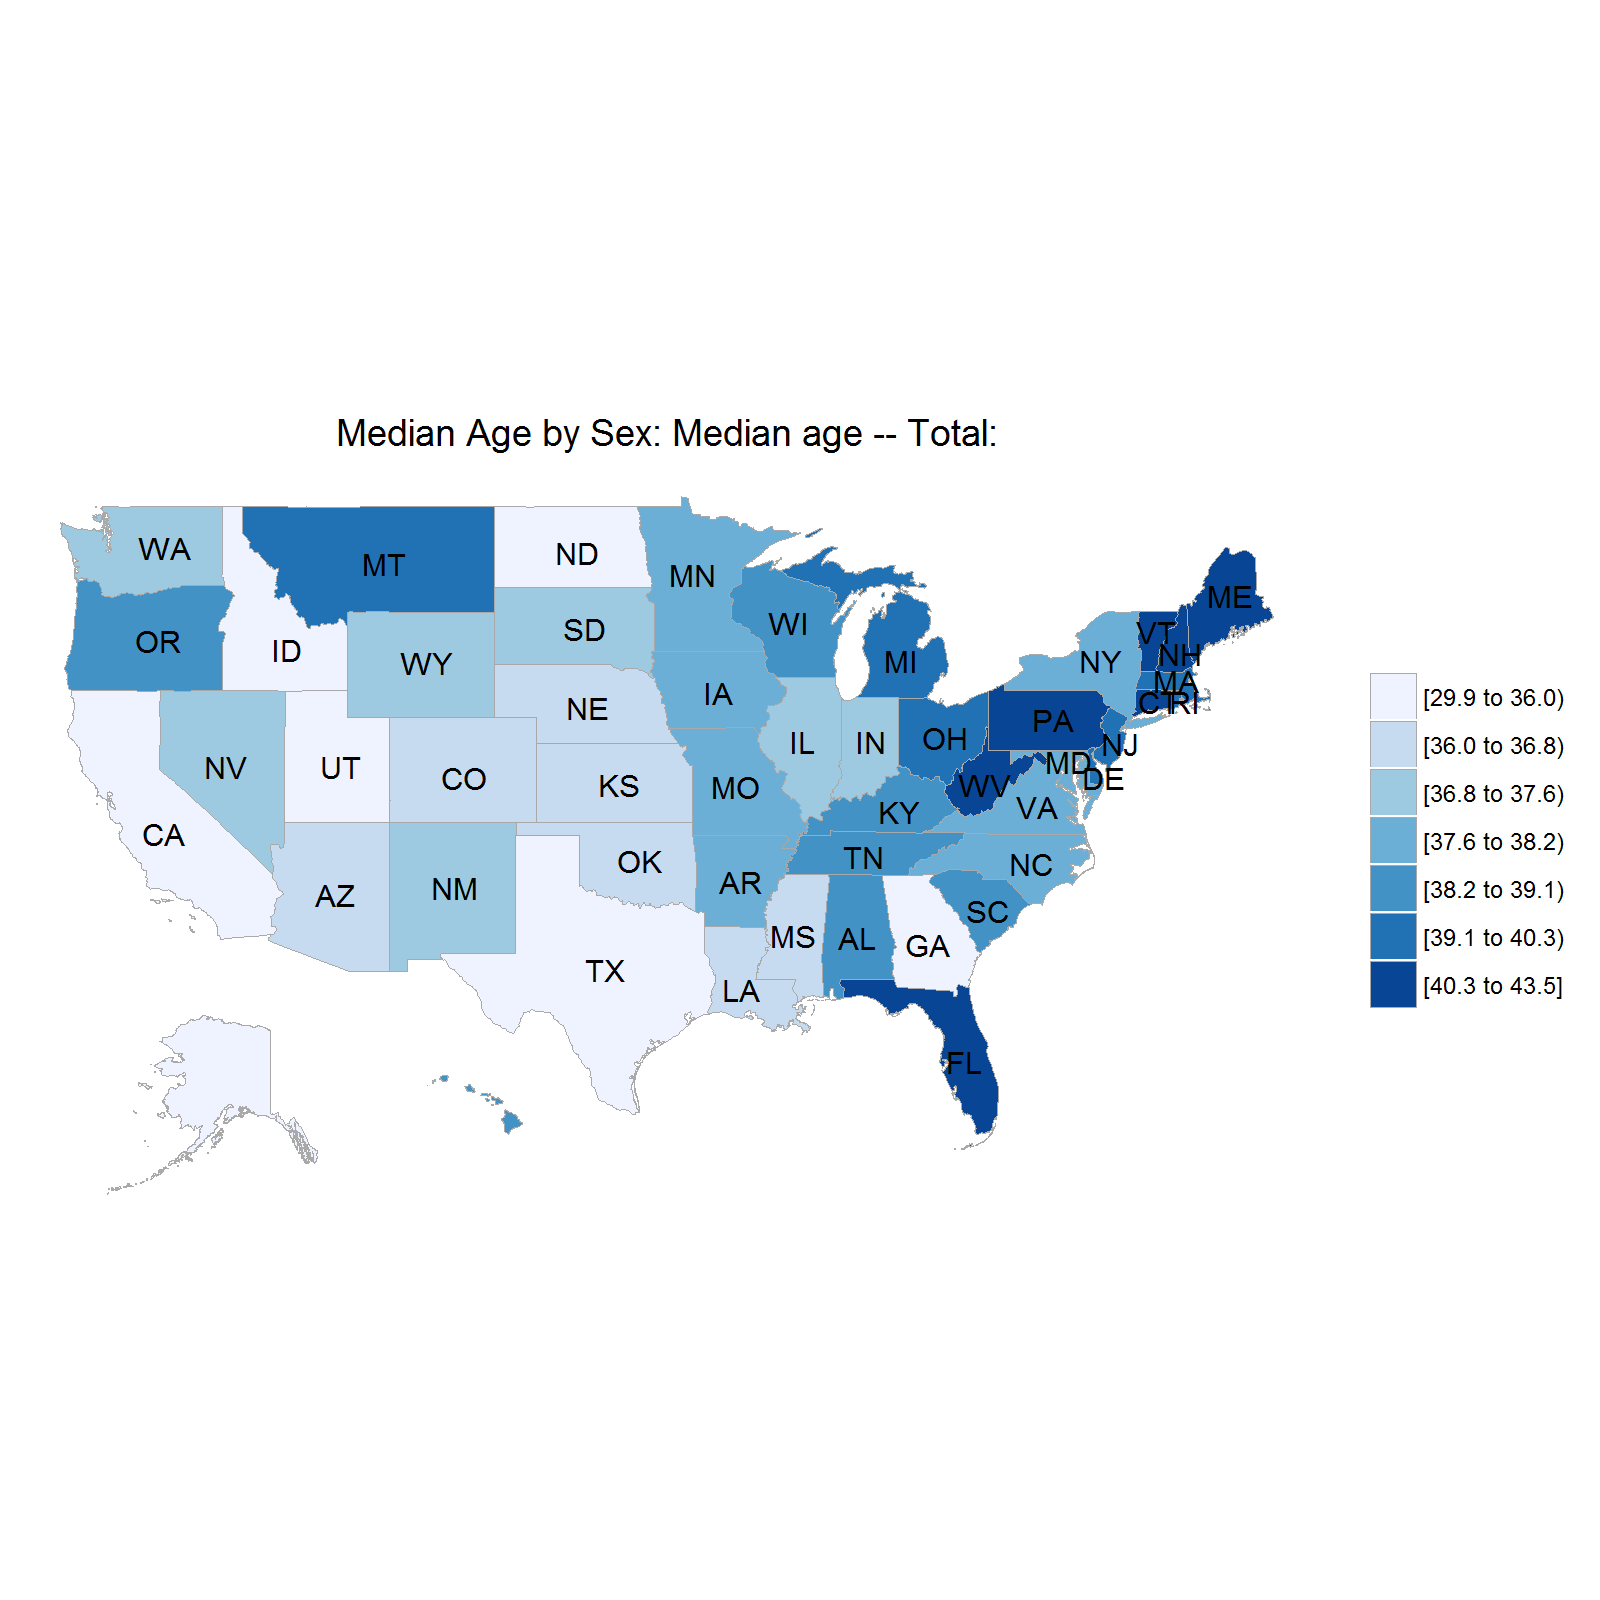
\includegraphics[height=12.50000in]{images/state_age.png}}{US Median Age by State}}\label{us-median-age-by-state}

\newpage

\subsubsection{Figure B3 United States Average Income by
State}\label{figure-b3-united-states-average-income-by-state}

\section{\texorpdfstring{\protect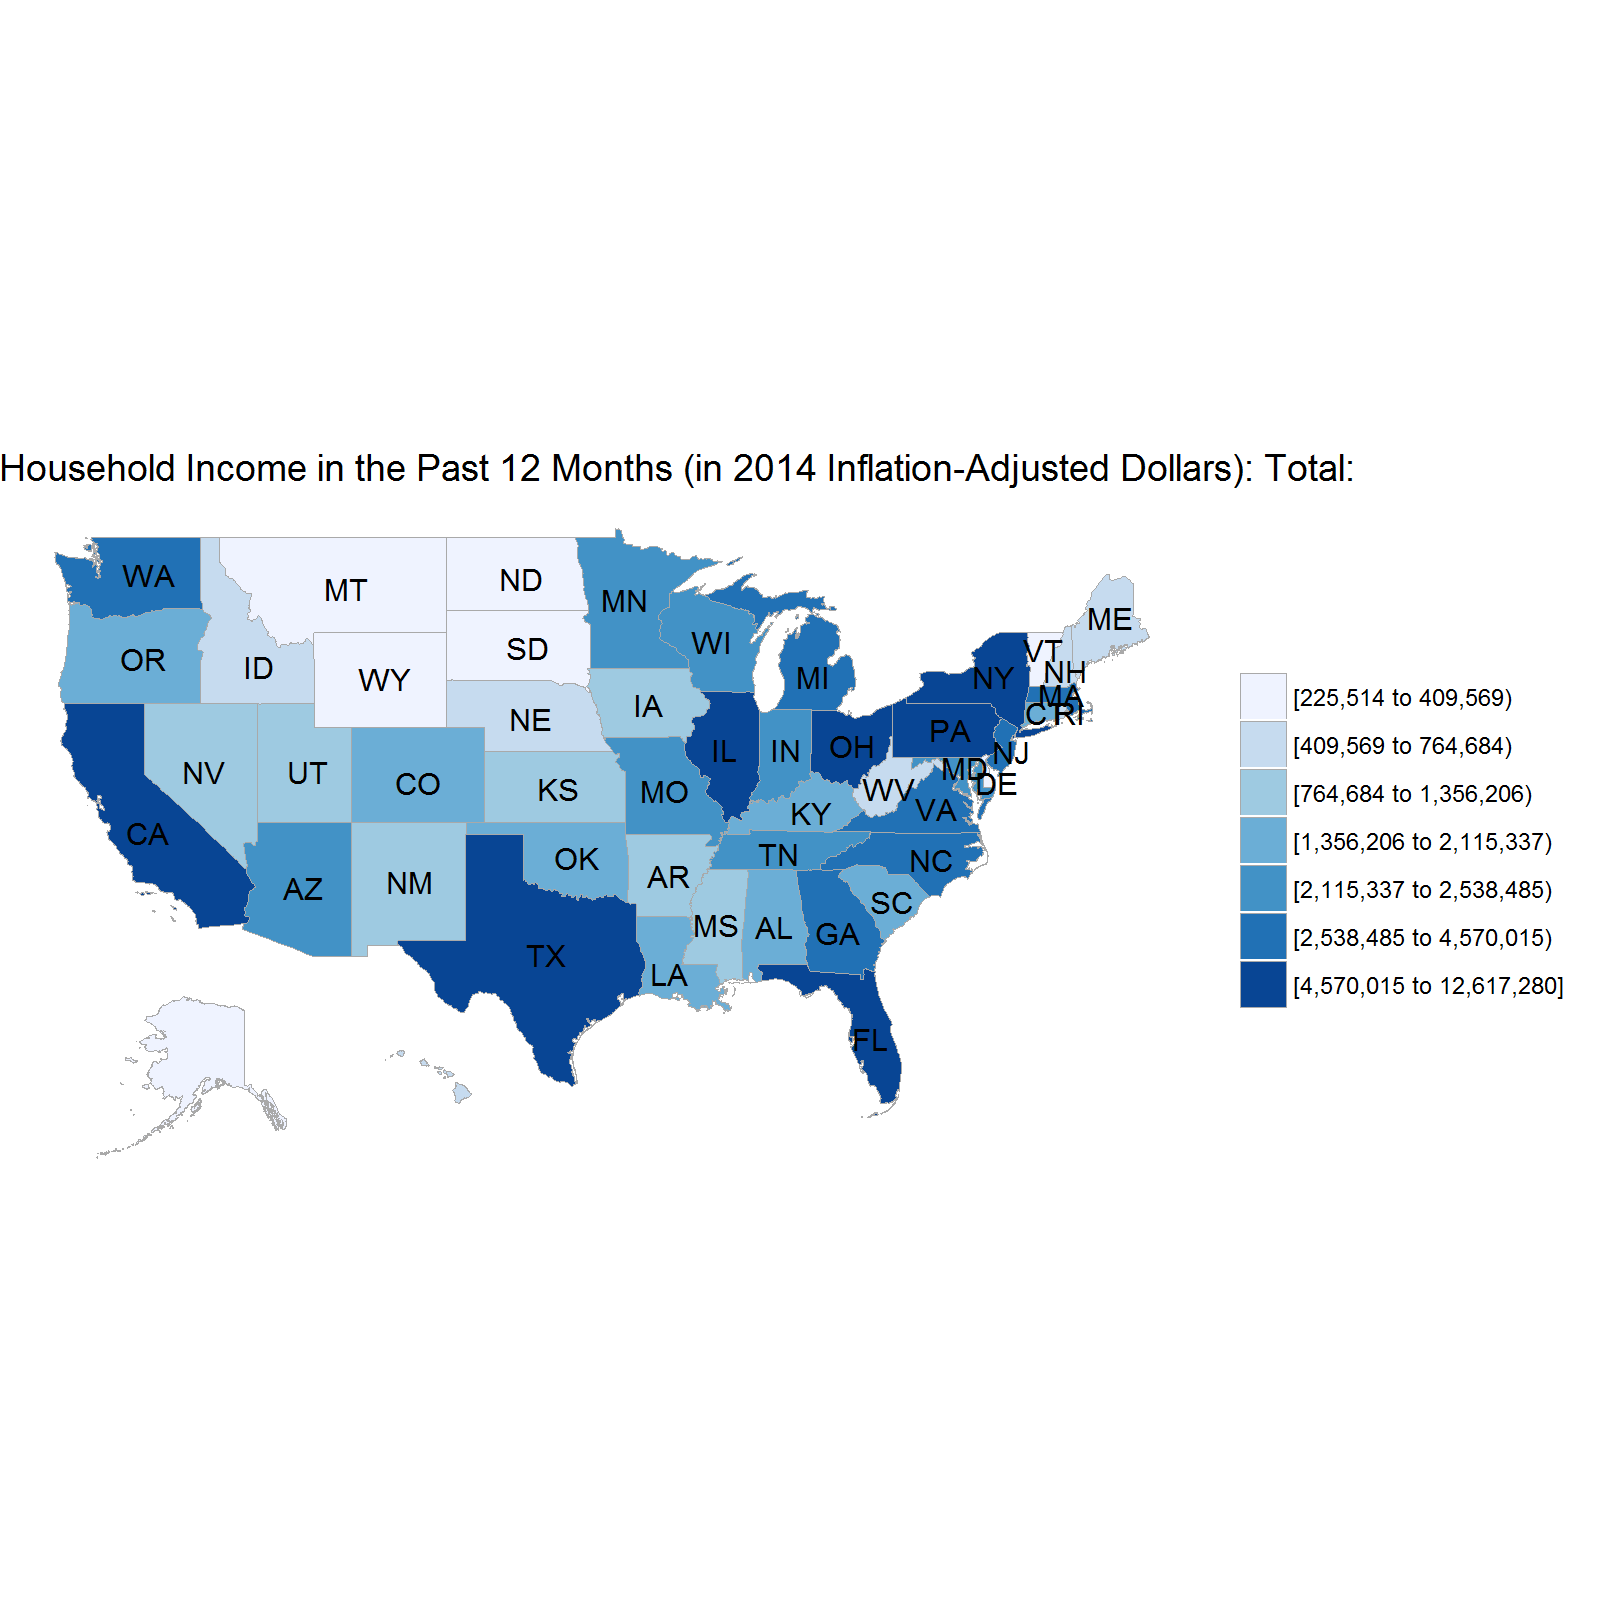
\includegraphics[height=12.50000in]{images/state_income.png}}{US Average Income by State}}\label{us-average-income-by-state}

\newpage

\subsubsection{Figure B4 United States Population by
County}\label{figure-b4-united-states-population-by-county}

\section{\texorpdfstring{\protect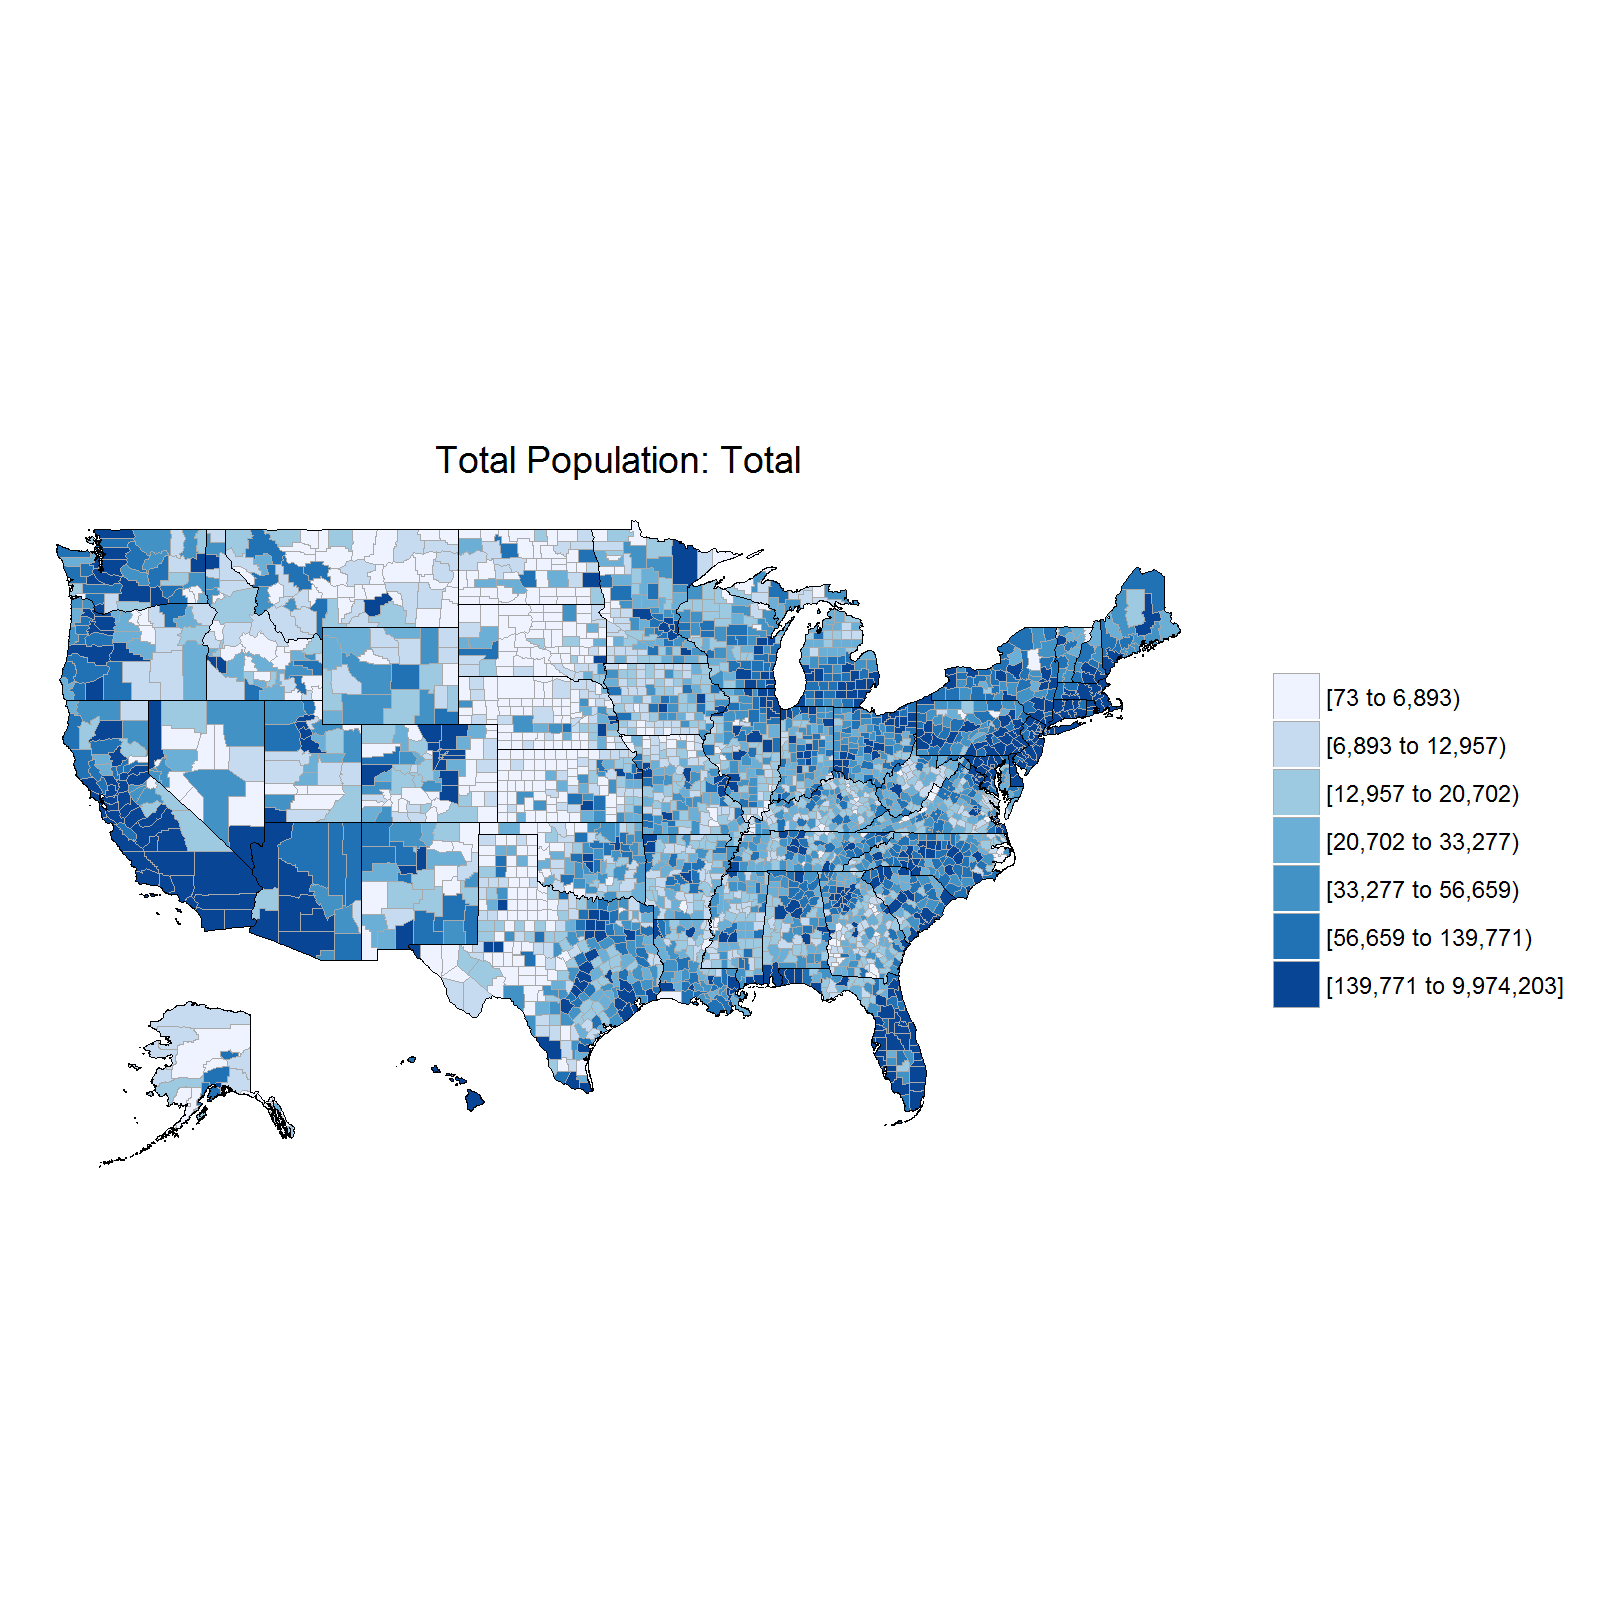
\includegraphics[height=12.50000in]{images/county_pop.png}}{US Population by County}}\label{us-population-by-county}

\newpage

\subsubsection{Figure B5 United States Median Age by
County}\label{figure-b5-united-states-median-age-by-county}

\section{\texorpdfstring{\protect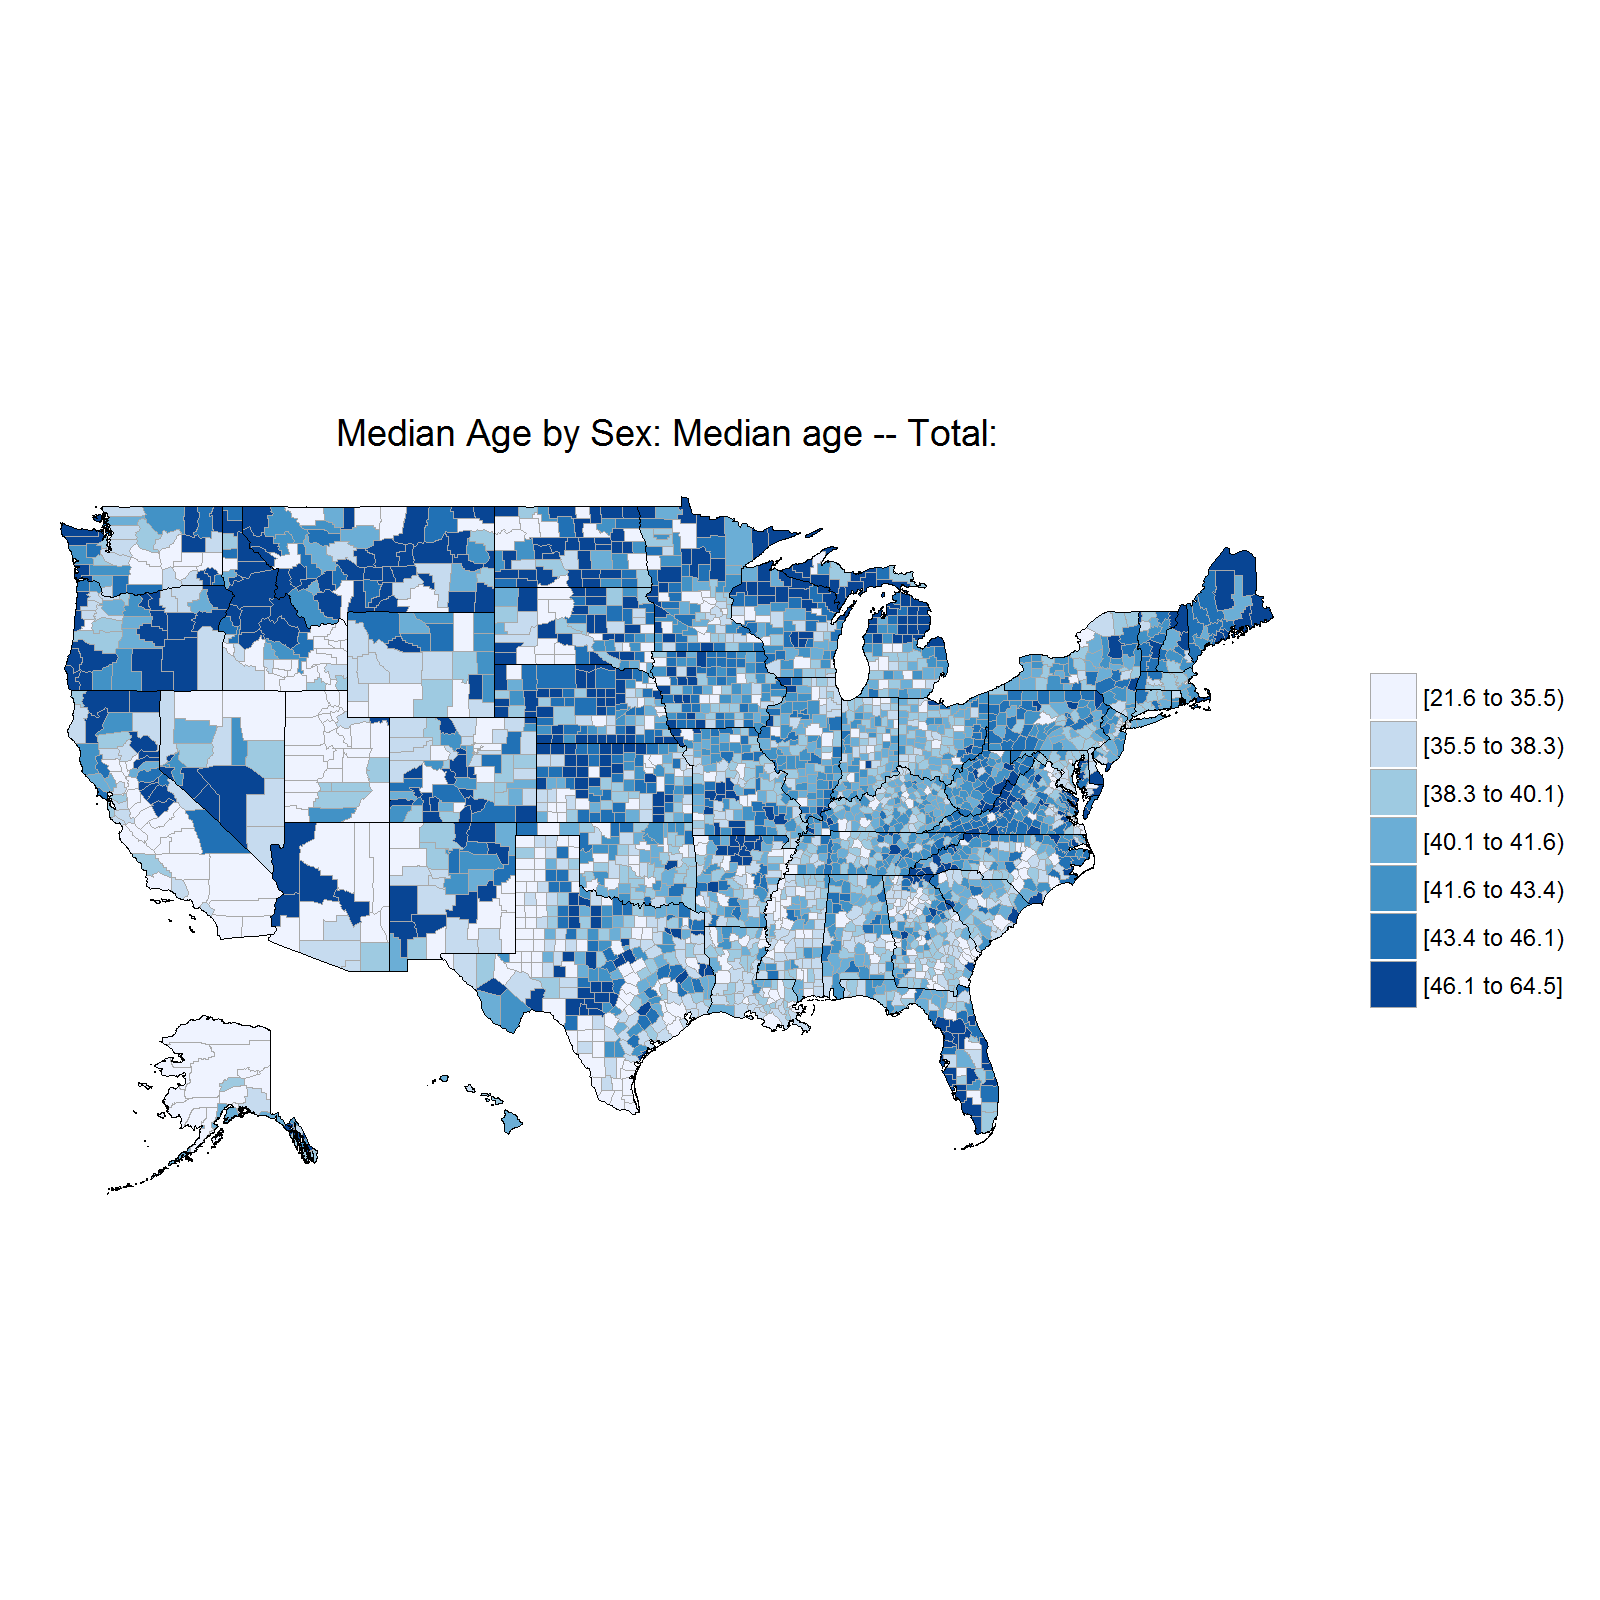
\includegraphics[height=12.50000in]{images/county_age.png}}{US Median Age by County}}\label{us-median-age-by-county}

\newpage

\subsubsection{Figure B6 United States Average Income by
County}\label{figure-b6-united-states-average-income-by-county}

\section{\texorpdfstring{\protect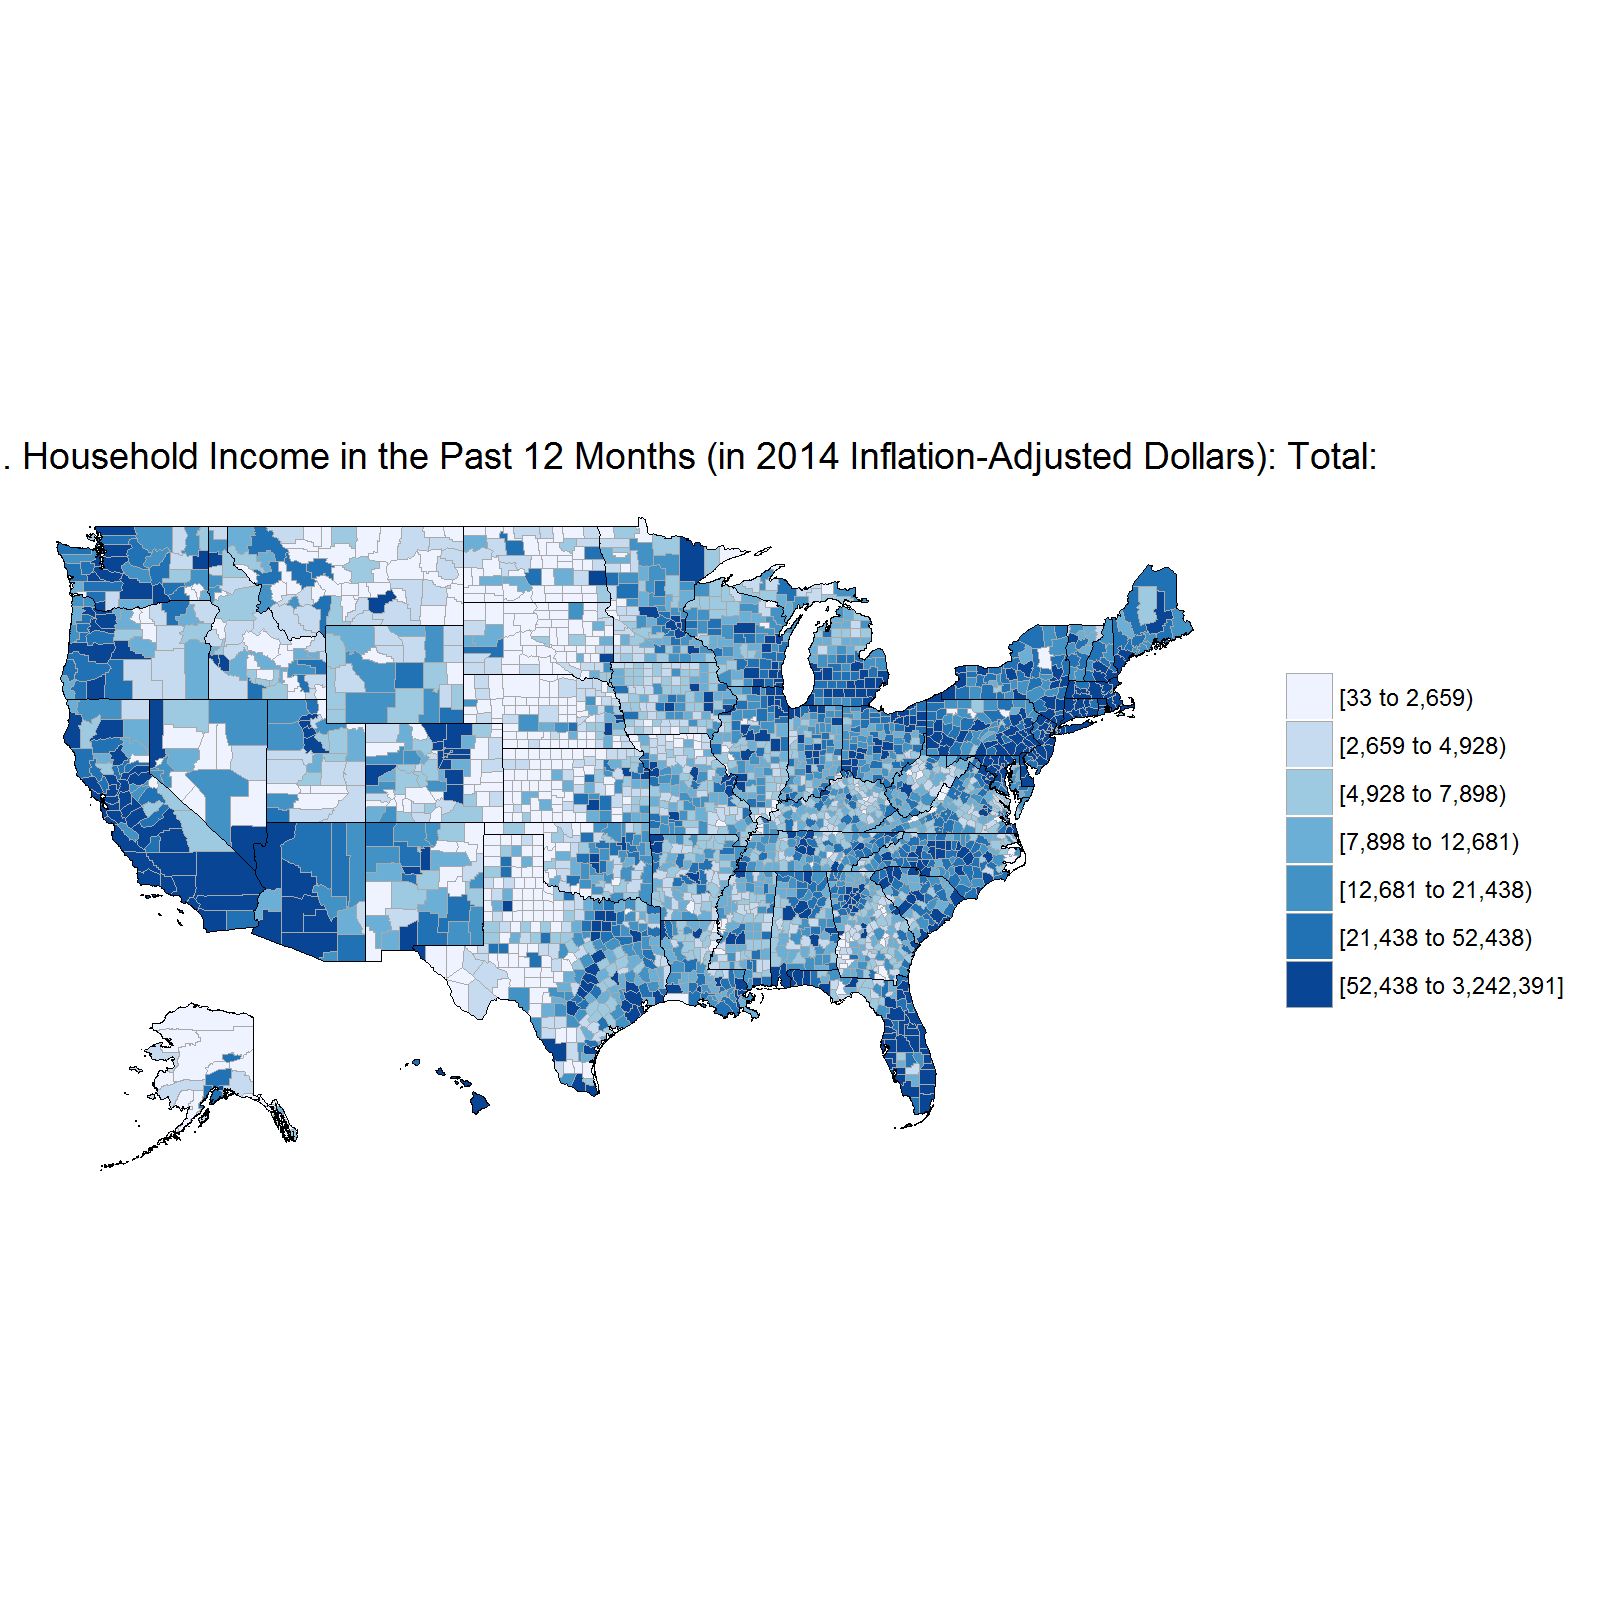
\includegraphics[height=12.50000in]{images/county_income.png}}{US Average Income by County}}\label{us-average-income-by-county}

\newpage

\subsubsection{Figure B7 United States High/Low Income by
County}\label{figure-b7-united-states-highlow-income-by-county}

\section{\texorpdfstring{\protect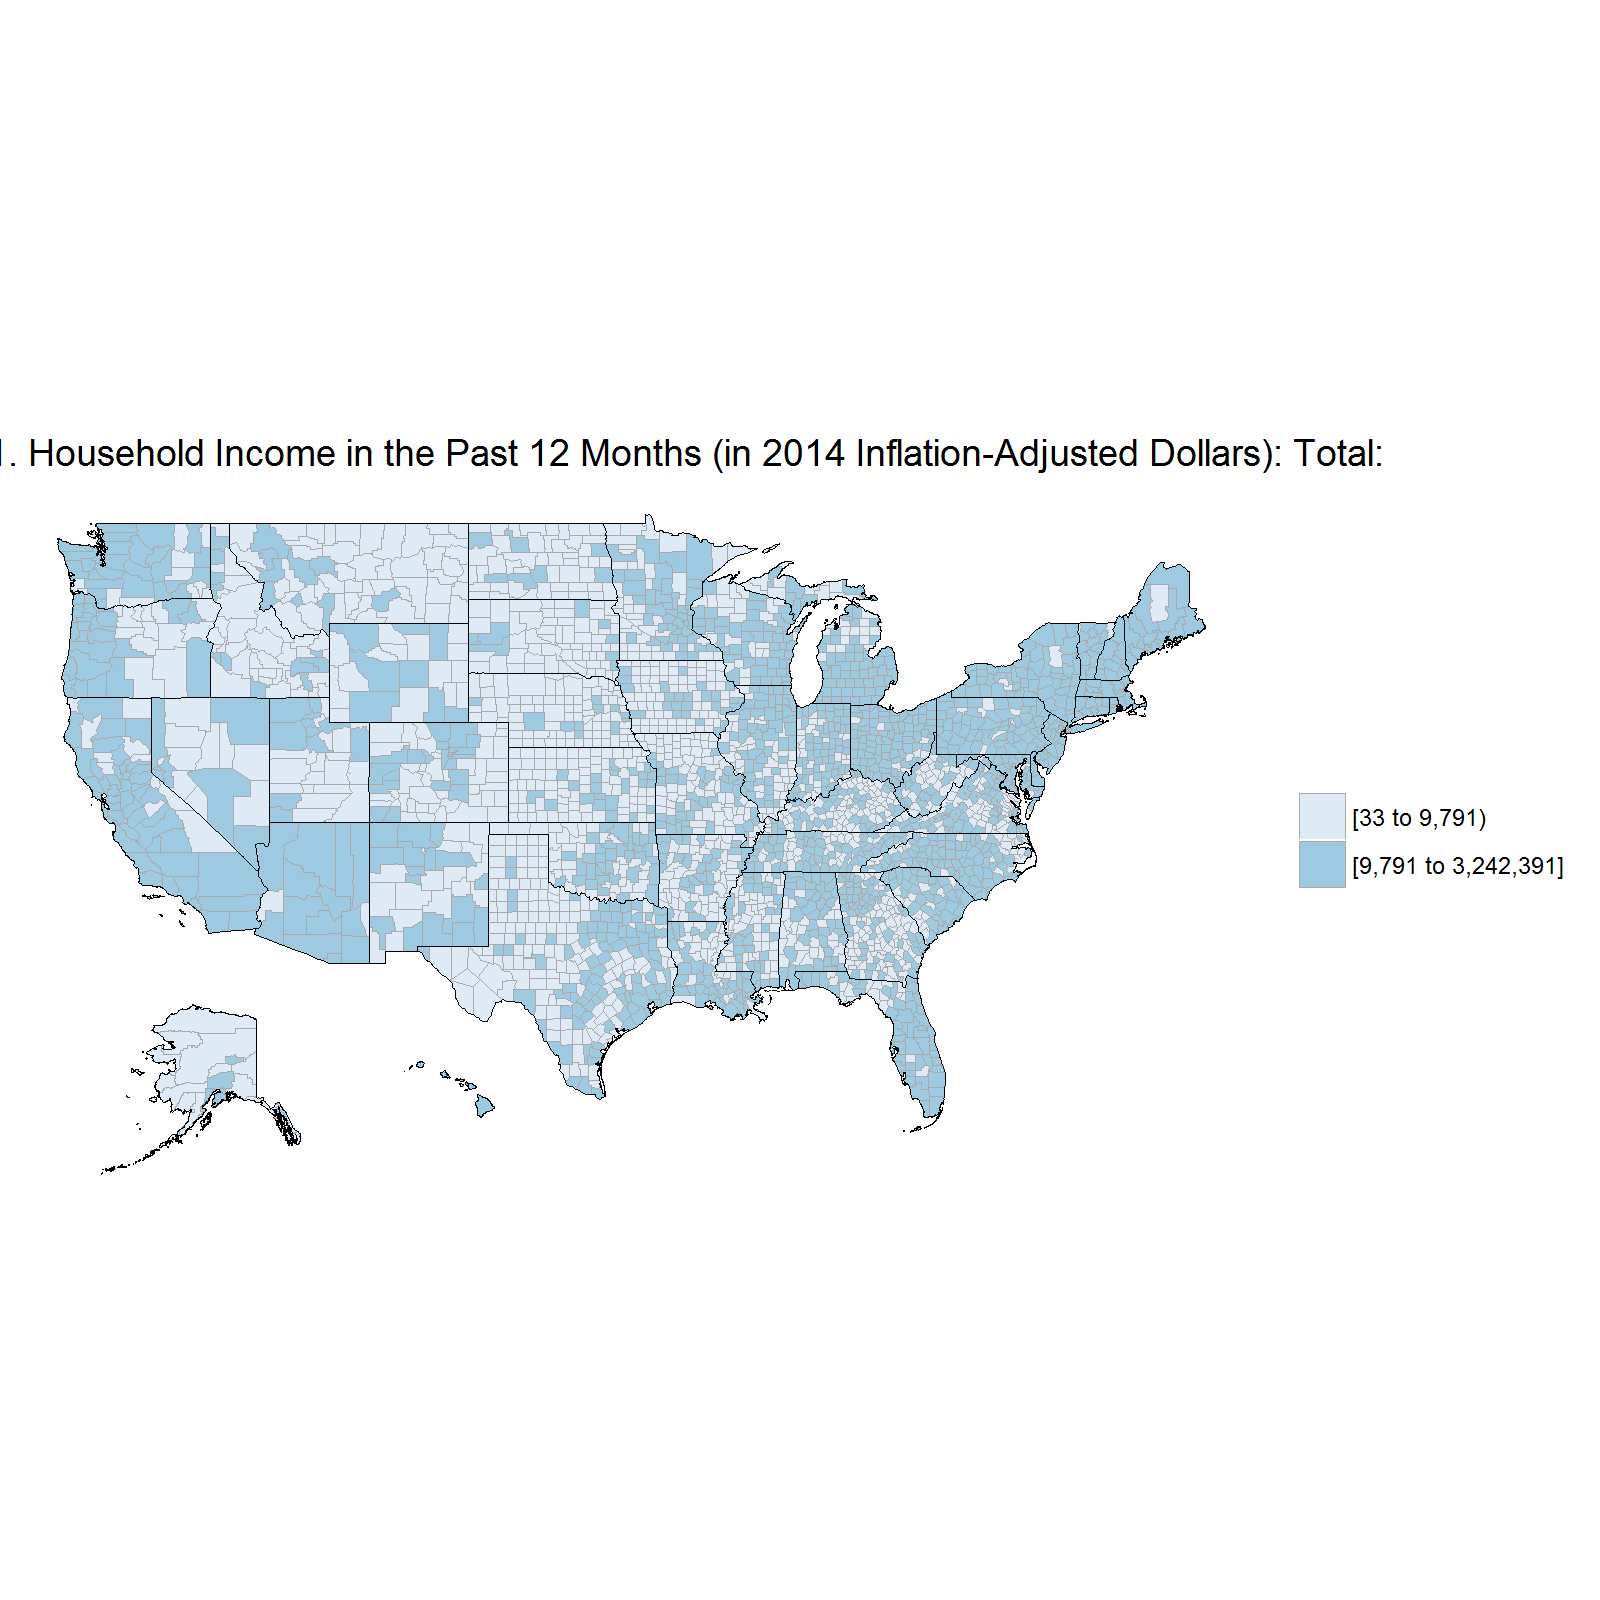
\includegraphics[height=12.50000in]{images/county_income_twolvl.png}}{US High/Low Income by County}}\label{us-highlow-income-by-county}

\newpage

\subsubsection{Figure B8 United States Average Income by
County}\label{figure-b8-united-states-average-income-by-county}

\section{\texorpdfstring{\protect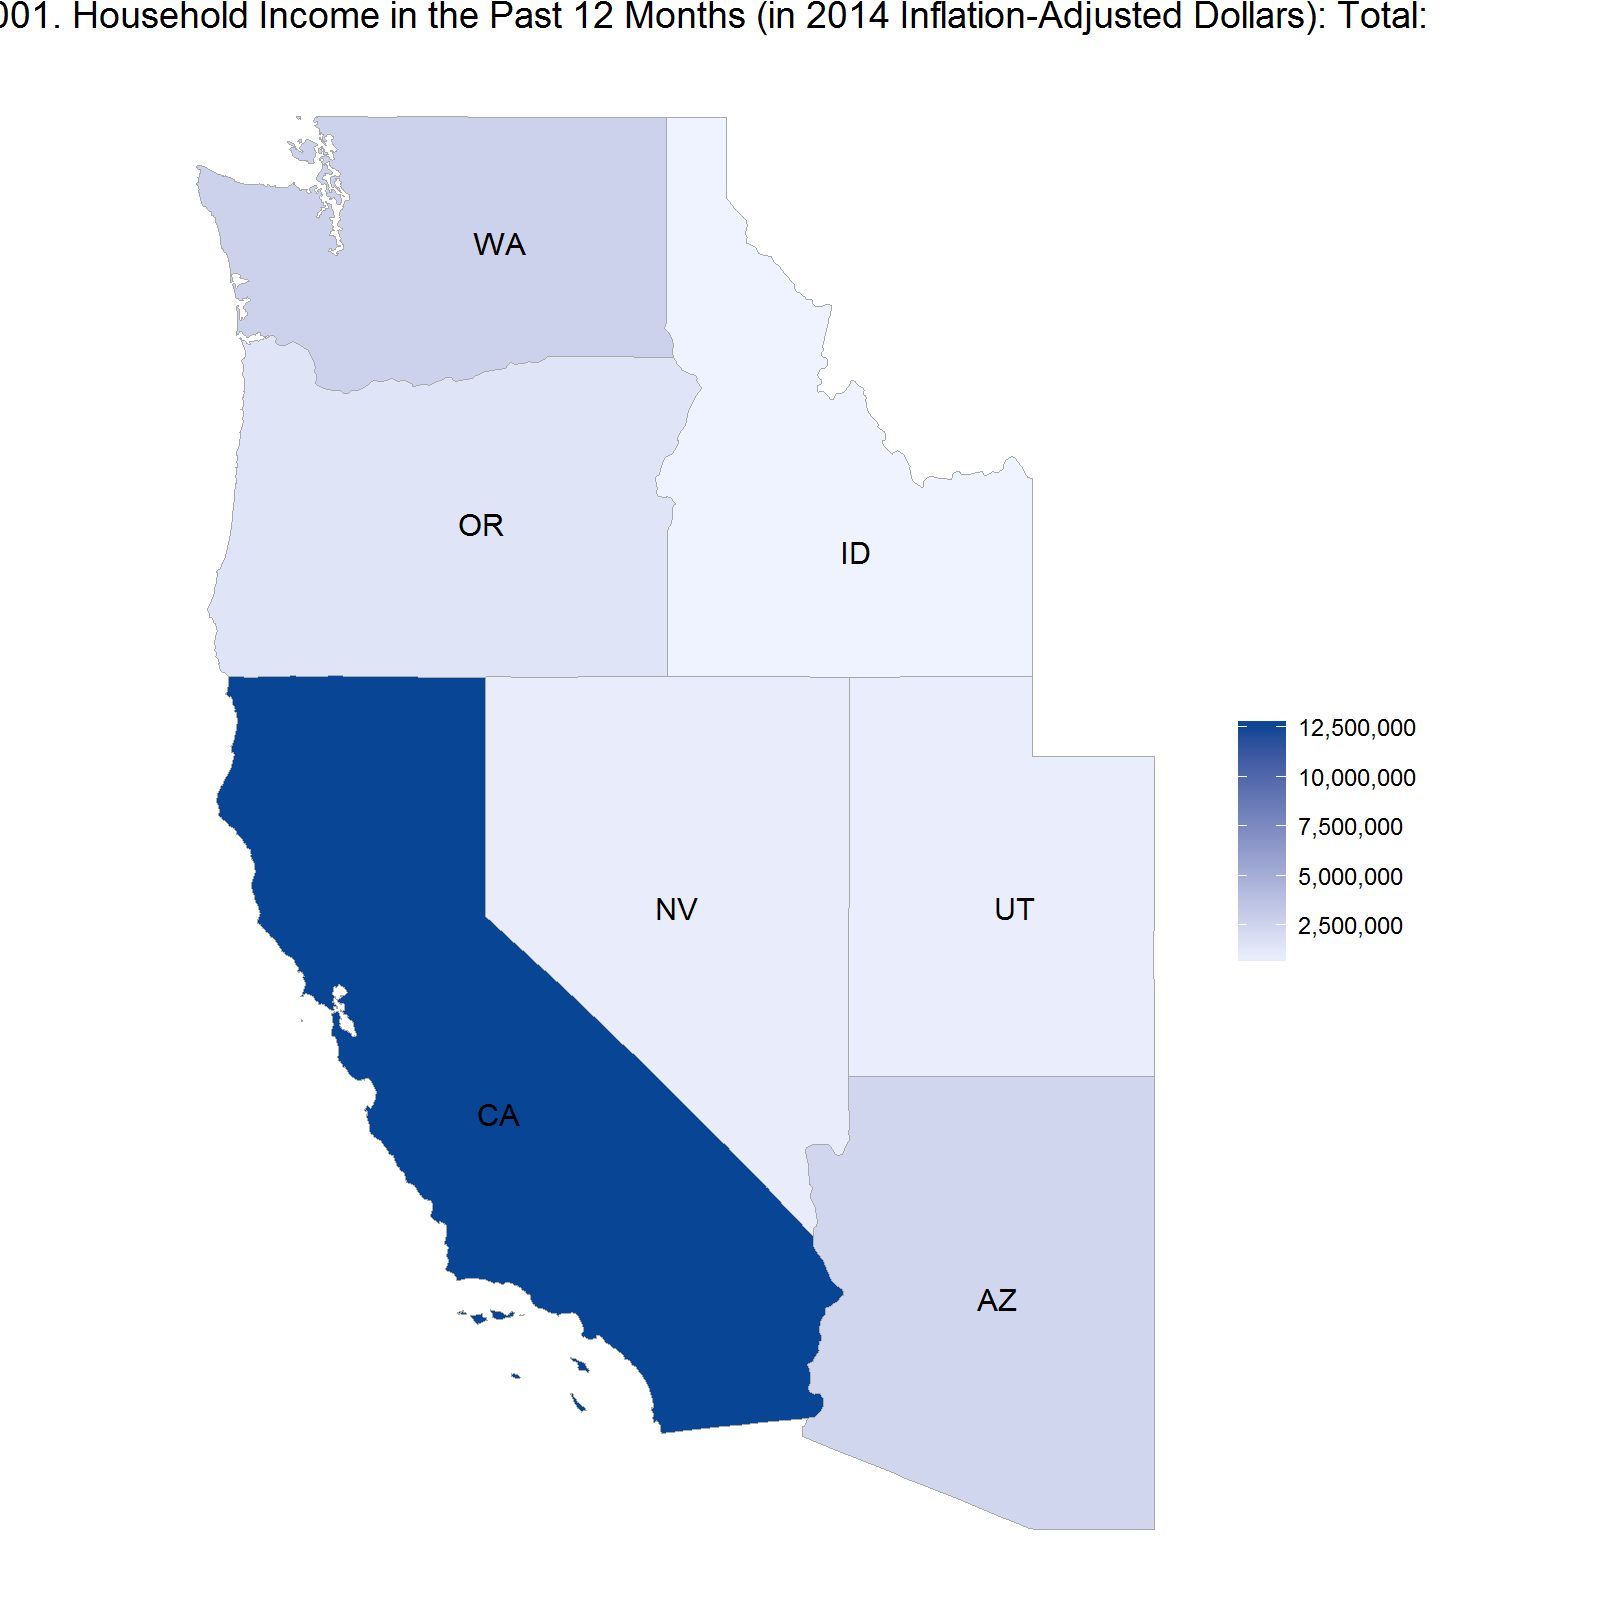
\includegraphics[height=12.50000in]{images/county_income_wczoom.png}}{US Average Income by County}}\label{us-average-income-by-county-1}

\newpage

\section*{References}\label{references}
\addcontentsline{toc}{section}{References}

\hypertarget{refs}{}
\hypertarget{ref-ACS2014}{}
Commerce, U.S. Department of. 2015. ``American Community Survey.''
\url{https://www.census.gov/acs/www/}.

\hypertarget{ref-tru2014}{}
Innovation, Truila Tech \&. 2014. ``The Choroplethr Package for R.''
\url{http://www.trulia.com/blog/tech/the-choroplethr-package-for-r/}.


\end{document}
